\documentclass[a4paper,11pt]{article}
\usepackage[T1]{fontenc}
\usepackage[utf8]{inputenc}
\usepackage{lmodern}
\usepackage{graphicx}
\usepackage{amsmath}
\usepackage{amsfonts}
\usepackage{amssymb}
\usepackage{mathtools}
\usepackage{epstopdf}

\DeclareMathOperator{\given}{\mid}
\DeclareMathOperator*{\argmax}{argmax}
\DeclareMathOperator*{\argmin}{argmin}

\begin{document}

\section*{HW4}

\begin{tabular*}{0.9\textwidth}{@{\extracolsep{\fill} } lll}
Jimmy Hold\"{o} & & Jared Karr\\
890130-6319 & & 801120-4693\\
\it{gusholji@student.gu.se} & & \it{karr@student.chalmers.se}\\
\end{tabular*}
%%%%%%%%%%%%%%%%%%%%%%%%%%%%%%%%%%%%%%%%
%%%%%%%%%%%%%%%%%%%%%%%%%%%%%%%%%%%%%%%%
\section{Theoretical problems}
%%%%%%%%%%%%%%%%%%%%%%%%%%%%%%%%%%%%%%%%
\subsection{SVM}
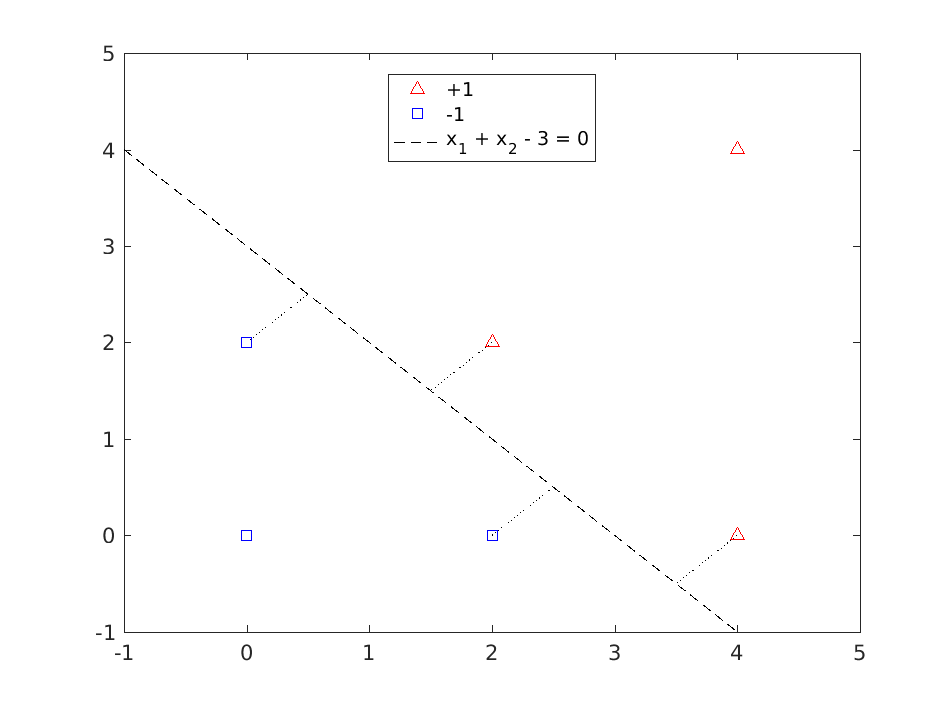
\includegraphics[width=\textwidth]{P1_1}
\begin{align*}
  2\gamma = 2\frac{\mid2\cdot1+2\cdot1-3\mid}{\sqrt{1^2+1^2}} = \sqrt{2}
\end{align*}
%%%%%%%%%%%%%%%%%%%%%%%%%%%%%%%%%%%%%%%%
\subsection{SVM cont'd}
\paragraph{(a)}
\begin{align*}
  (\hat{w}_1,\hat{w}_2)
  =\argmin_{(w_1,w_2)}w_1^2+w_2^2
\end{align*}
subject to constraints
\begin{alignat}{4}
  2w_1 &+& 2w_2 &+& b &\ge& 1\label{eq:p1}\\
  4w_1 &+& 4w_2 &+& b &\ge& 1\label{eq:p2}\\
  4w_1 & &      &+& b &\ge& 1\label{eq:p3}\\
       & &      & &-b &\ge& 1\label{eq:p4}\\
 -2w_1 & &      & &-b &\ge& 1\label{eq:p5}\\
       & &-2w_2 & &-b &\ge& 1\label{eq:p6}
\end{alignat}

\paragraph{(b)}
Combine constraints
\begin{align*}
  2w_1&\ge2 & w_1&\ge1 \tag*{\eqref{eq:p1} and \eqref{eq:p6}}\\
  2w_2&\ge2 & w_2&\ge1 \tag*{\eqref{eq:p1} and \eqref{eq:p5}}\\
    -b&\ge3 &   b&\le-3 \tag*{\eqref{eq:p1}, \eqref{eq:p5} and \eqref{eq:p6}}
\end{align*}
The solution $\hat{w}_1=1, \hat{w}_2=1, \hat{b}=-3$ satisfies the constraints \eqref{eq:p2}, \eqref{eq:p3} and \eqref{eq:p4}.

\paragraph{(c)}
\begin{multline}
  \hat{\boldsymbol{\alpha}}=
  \argmax_{\boldsymbol{\alpha}}\sum_{n=1}^6\alpha_n
    -4\alpha_1^2
    -16\alpha_1\alpha_2
    -8\alpha_1\alpha_3
    +4\alpha_1\alpha_5
    +4\alpha_1\alpha_6
    -16\alpha_2^2\\
    -16\alpha_2\alpha_3
    +8\alpha_2\alpha_5
    +8\alpha_2\alpha_6
    -8\alpha_3^2
    +8\alpha_3\alpha_5
    -2\alpha_5^2
    -2\alpha_6^2\label{eq:dual}
\end{multline}
subject to constraints
\begin{align*}
\alpha_1+\alpha_2+\alpha_3-\alpha_4-\alpha_5-\alpha_6=0,\qquad\alpha_n\ge0
\end{align*}
\paragraph{(d)}
%%%%%%%%%%%%%%%%%%%%%%%%%%%%%%%%%%%%%%%%
%%%%%%%%%%%%%%%%%%%%%%%%%%%%%%%%%%%%%%%%
\section{Practical problems}
%%%%%%%%%%%%%%%%%%%%%%%%%%%%%%%%%%%%%%%%
\subsection{SVM}

%%%%%%%%%%%%%%%%%%%%%%%%%%%%%%%%%%%%%%%%
\subsection{Kernels}
\end{document}
